\documentclass[tikz,border=3pt]{standalone}
\usetikzlibrary{arrows.meta,decorations.markings}
\begin{document}
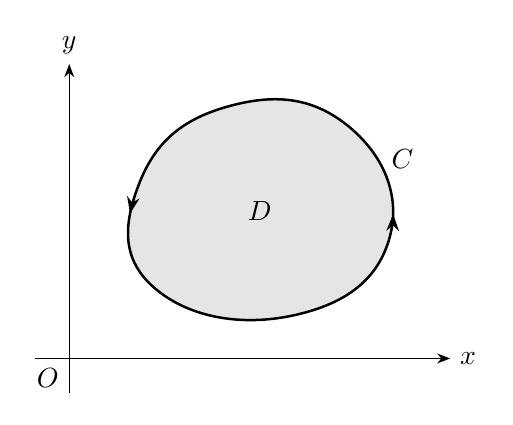
\begin{tikzpicture}[scale=1.1,>=Stealth,line width=0.9pt,
  mid/.style={postaction={decorate},decoration={markings,mark=at position #1 with {\arrow{Stealth[length=6pt]}},mark=at position #1+0.5 with {\arrow{Stealth[length=6pt]}}}}]
  \draw[line width=0.4pt,->] (-0.4,0) -- (4.4,0) node[right] {$x$};
  \draw[line width=0.4pt,->] (0,-0.4) -- (0,3.4) node[above] {$y$};
  \draw[fill=black!10,mid=0.2] plot[smooth cycle,tension=0.8] coordinates {(1,0.8) (2.6,0.5) (3.7,1.4) (3.2,2.7) (1.8,2.9) (0.8,2.0)};
  \node at (2.2,1.7) {$D$};
  \node[right] at (3.6,2.3) {$C$};
  \node[below left] at (0,0) {$O$};
\end{tikzpicture}
\end{document}
